% ============================================
%  Article Class (This is a LaTeX2e document)
% ============================================
\documentclass[12pt]{scrartcl}
\usepackage[english]{babel}
\usepackage[round]{natbib}
\usepackage[T1]{fontenc}
\usepackage{color}

% ============================
%  Figures and relative paths
% ============================
\usepackage{graphicx}
\graphicspath{{figures/}}

% =======================
%  References to classes
% =======================
\usepackage[colorlinks=true]{hyperref}
\newcommand{\rbametabolism}{\hyperref[sec:rba_metabolism]{\textbf{RBAMetabolism}}}
\newcommand{\compartment}{\hyperref[sec:compartment]{\textbf{Compartment}}}
\newcommand{\species}{\hyperref[sec:species]{\textbf{Species}}}

% ==========
%  Document
% ==========
\begin{document}

\title{XML format for RBA models}
\author{S. Fischer, V. Fromion, A. Goelzer}
\date{\today}

\maketitle

\newpage

\tableofcontents

\newpage

\section{Introduction}

In this document we present the XML structures used to define a RBA model.
A complete RBA model is composed of the following files:
\begin{itemize}
  \item metabolism.xml
  (definition of compartments, metabolic species and metabolic reactions).
  \item parameters.xml
  (definition of density constraints and user-defined functions).
  \item proteins.xml (definition of proteins).
  \item rnas.xml (definition of RNAs).
  \item dna.xml (definition of DNA).
  \item enzymes.xml
  (definition of enzymatic machineries catalyzing metabolic reactions).
  \item processes.xml
  (definition of cell processes necessary to growth and maintenance).
\end{itemize}

For every file, we present the nodes that composes the XML structure.
For every node, we show a class diagram that shows the node's attributes
and the children node that it may/must contain.
We provide a brief description about the relevance of the node
in the RBA model.


\section{Conventions}

\subsection{Naming conventions}

\subsection{Boolean attributes}


\section{metabolism.xml}

\subsection{RBAMetabolism container}

The metabolism file is strongly inspired by SBML.\@
More precisely, it is a subpart of an SBML file.

\subsubsection{RBAMetabolism}
\label{sec:rba_metabolism}

The outermost portion of the metabolism file is an instance of class
\rbametabolism, shown in Figure~\ref{fig:metabolism_doc}.

\begin{figure}
  \centering
  \includegraphics[scale=0.9]{figures/metabolism_doc}
  \caption{XML structure of metabolism document.}
\label{fig:metabolism_doc}
\end{figure}

Currently, \rbametabolism{} has no simple attributes.
It includes exactly one instance of \textbf{ListOf} container classes.
All \textbf{ListOf} classes do not have own attributes,
they are merely used to organize a list of instances from another class.
This organization was inspired by SBML.\@

\subsubsection{Compartment}
\label{sec:compartment}

The \compartment{} class is used to list existing cell compartments.

\paragraph{The \textit{id} attribute}
The \textbf{id} attribute is a string defining the identifier of a compartment.

\subsubsection{Species}
\label{sec:species}

The \species{} class is used to list \emph{metabolic} species.

\paragraph{The \textit{id} attribute}
The \textbf{id} attribute is a string defining the identifier of a metabolite.

\paragraph{The \textit{boundaryCondition} attribute}
The \textbf{boundaryCondition} attribute is a boolean.
If the attribute is set to true, the metabolite is considered to be at
a constant concentration.
In other words, it is not affected by reactions.
This is typical for metabolites in the external medium.


\section{parameters.xml}

\subsection{RBAMetabolism container}

The metabolism file is strongly inspired by SBML.\@
More precisely, it is a subpart of an SBML file.

\subsubsection{RBAMetabolism}
\label{sec:rba_metabolism}

The outermost portion of the metabolism file is an instance of class
\rbametabolism, shown in Figure~\ref{fig:metabolism_doc}.

\begin{figure}
  \centering
  \includegraphics[scale=0.9]{figures/metabolism_doc}
  \caption{XML structure of metabolism document.}
\label{fig:metabolism_doc}
\end{figure}

Currently, \rbametabolism{} has no simple attributes.
It includes exactly one instance of \textbf{ListOf} container classes.
All \textbf{ListOf} classes do not have own attributes,
they are merely used to organize a list of instances from another class.
This organization was inspired by SBML.\@

\subsubsection{Compartment}
\label{sec:compartment}

The \compartment{} class is used to list existing cell compartments.

\paragraph{The \textit{id} attribute}
The \textbf{id} attribute is a string defining the identifier of a compartment.

\subsubsection{Species}
\label{sec:species}

The \species{} class is used to list \emph{metabolic} species.

\paragraph{The \textit{id} attribute}
The \textbf{id} attribute is a string defining the identifier of a metabolite.

\paragraph{The \textit{boundaryCondition} attribute}
The \textbf{boundaryCondition} attribute is a boolean.
If the attribute is set to true, the metabolite is considered to be at
a constant concentration.
In other words, it is not affected by reactions.
This is typical for metabolites in the external medium.



\end{document}
% ----------------------------------------------------------------
